\section{Fluid Rendering}


\noindent
Rendering a fluid requires a few preprocessing steps to merge nearby particles, creating a semi-smooth surface for which we can compute normals and, subsequently, refraction and reflection vectors. One key limitation of this approach is that we only compute surfaces \textit{visible} from the camera, which means that information about occluded surfaces is discarded. This implies that only the first refraction/reflection vector is computed, leading to visually plausible, albeit physically inaccurate, light distortions.

\begin{figure}[ht!]
    \centering
        \subfloat{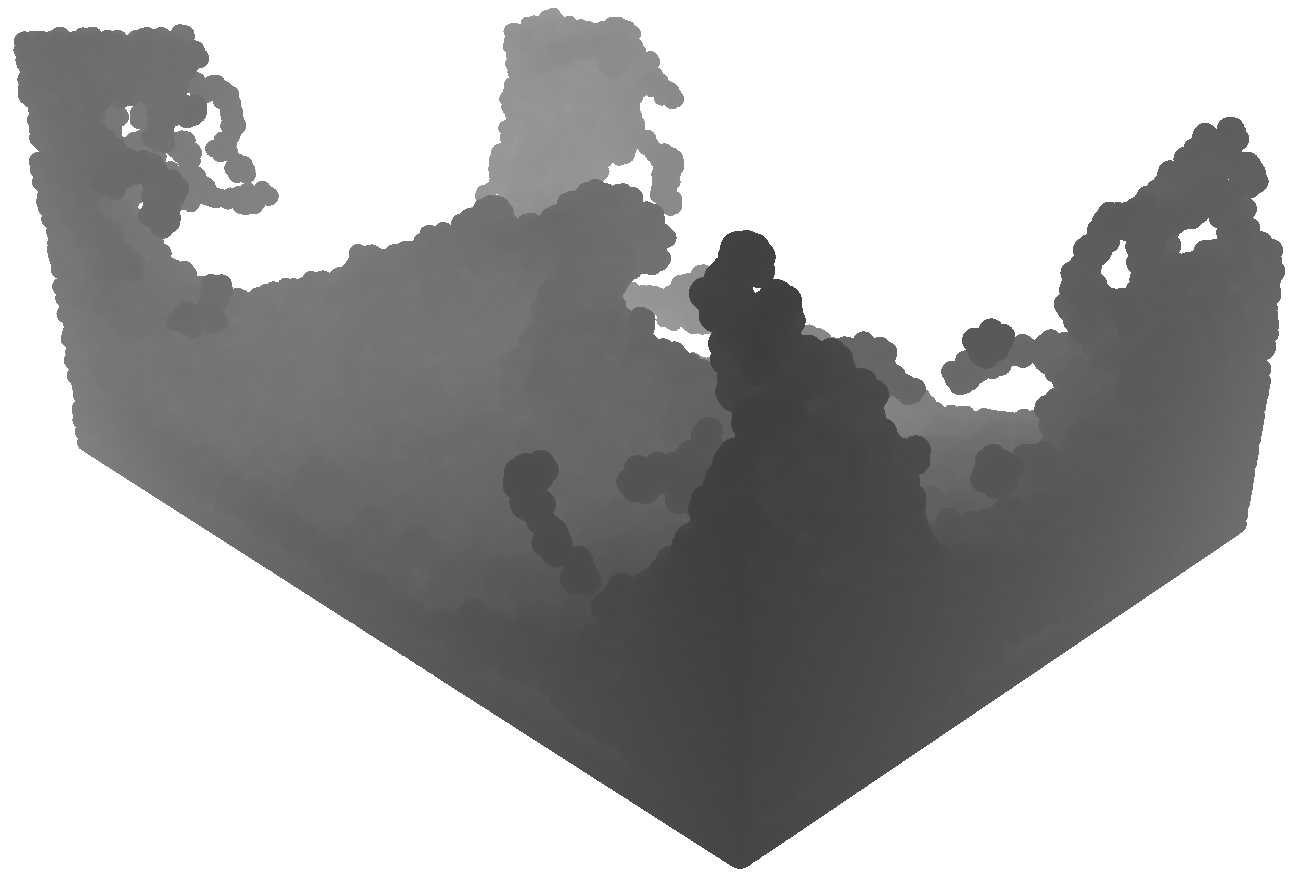
\includegraphics[width=.65\linewidth]{images/depthMap.png}}
    \caption{Per‑particle depth map.}\label{fig:depthmaps}
\end{figure}

\noindent
The first step consists of computing and storing a linear particle depthmap in a texture, as shown in Fig.\ref{fig:depthmaps}. This depthmap is used to filter out all those fragments not directly visible from the camera and, in later stages, becomes essential for reconstructing world-space coordinates from clip-space ones.

\noindent
To render the depthmap, we used a bigger particle radius, in order to have a greater overlap between particles, making it easier to smooth them. To compute the correct sphere surface depth, we used the same approach used in Eq.\ref{eq:sphereEq}.

\begin{figure}[ht!]
    \centering
        \subfloat[Original depth map]{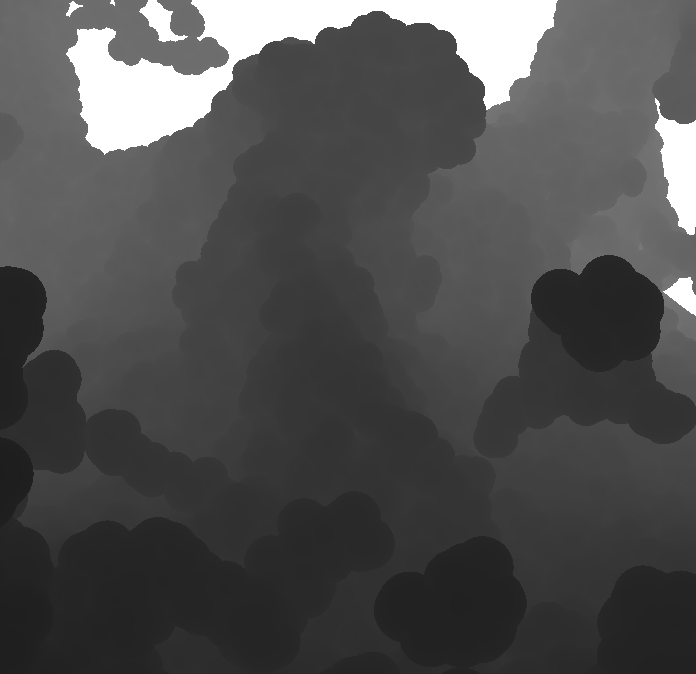
\includegraphics[width=.47\linewidth]{images/normals_plain.png}}\hfill
        \subfloat[Blurred depth map]{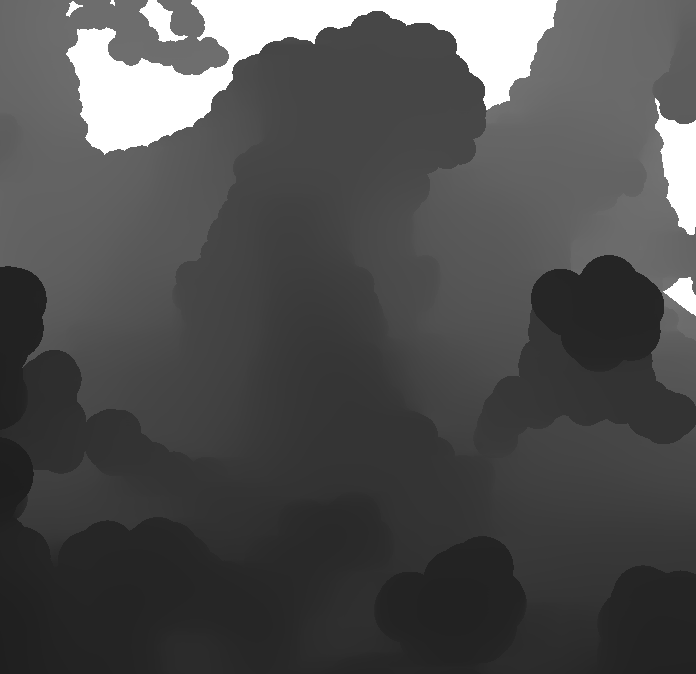
\includegraphics[width=.47\linewidth]{images/normals_blur.png}}
    \caption{Closeup of edge-preserving blurring applied to the depth map.}\label{fig:blurdepth}
\end{figure}

\noindent
In order to fuse together particles close to each other we used a two-pass bilateral filter, which is a type of edge-preserving smoothing filter, meaning that if there is an abrupt depth variation in the image (i.e. corresponding to an object's edge) it does not blur it, as shown in Fig. \ref{fig:blurdepth}.

\noindent
The filter works as follows:
\begin{itemize}
    \item \textbf{Vertical Pass:} the blurring only occurs on vertically adjacent texels and the resulting image is saved to a texture.
    \item \textbf{Horizontal Pass:} we blur horizontally adjacent texels, read from the vertical pass texture.
\end{itemize}

\noindent
The bilateral filter performs edge-preserving smoothing by computing each output pixel as a weighted average of its neighbors, where the weights are determined by both spatial proximity and photometric similarity. Specifically, pixels that are closer in spatial distance and have similar intensity values contribute more significantly, while those with large intensity differences have a reduced influence.
Formally, the formula for the 1D bilateral filter is:
\begin{align}
    w(i, j) &= \exp \left(-\frac{(i-j)^2}{2\sigma^2_d}-\frac{(p_i - p_j)^2}{2\sigma^2_r}\right) \label{eq:bilateralWeight}\\
    \hat{p_i} &= \frac{\sum_{j\in\Omega_i}p_j \cdot w(i,j)}{\sum_{j\in\Omega_i} w(i,j)}\label{eq:bilateralEqn}
\end{align}

\noindent
Here, $w(i,j)$ represents the weight assigned to the contribution of pixel $j$ when computing the final intensity of pixel $i$. In other words, $w(\cdot)$ is a kernel function -- specifically, a Gaussian kernel. The first term in Eq.\ref{eq:bilateralWeight} accounts for the spatial distance between pixels $i$ and $j$, while the second term weighs their intensity difference. The parameters $\sigma_d$ and $\sigma_r$ control the standard deviations of the spatial and range Gaussian kernels, respectively, determining their sensitivity to distance and intensity variations. In the implementation, these two parameters are named respectively \texttt{blurScale} and \texttt{blurFalloff}.\\
Finally, Eq.\ref{eq:bilateralEqn} defines the complete blurring operation for pixel $p_i$, where the output is computed as a weighted sum of the intensities of all neighboring pixels $j$, within the local window $\Omega_i$.\\

\noindent
Although computationally efficient, the separation of the horizontal and vertical blur passes introduces a few artifacts near the edges (which are clearly visible in the normal map in Fig.\ref{fig:normalMap}) but, in practice, are barely noticeable when the fluid is in motion.

\begin{figure}[ht!]
    \centering
        \subfloat{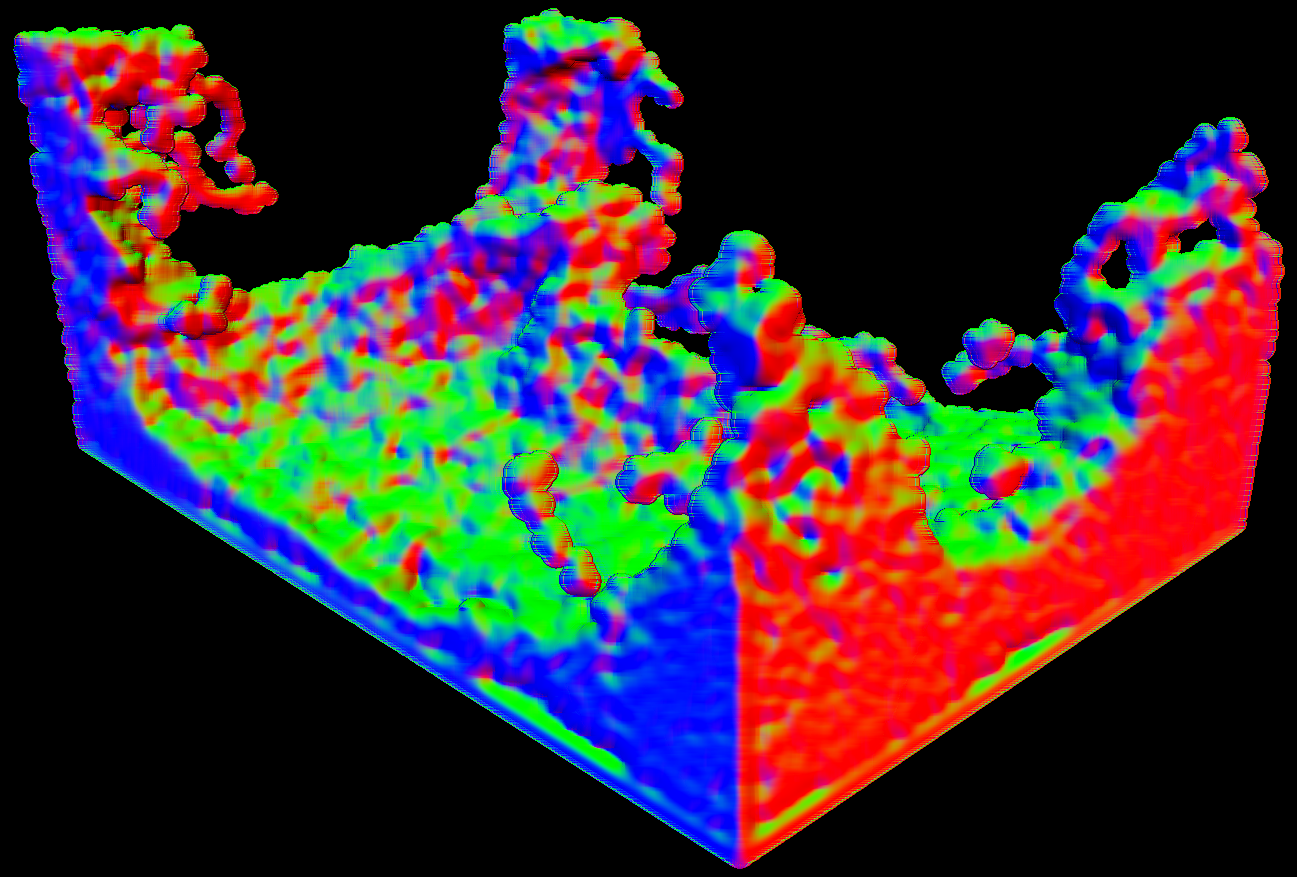
\includegraphics[width=.7\linewidth]{images/normalMap.png}}
    \caption{Normal map computed on the blurred depth map.}\label{fig:normalMap}
\end{figure}

\noindent
Normal reconstruction is performed by computing the cross product of two orthogonal displacement vectors, computed with respect to a $UV$ texture coordinate, as shown in the following algorithm:
\begin{algorithm}[H]
\caption{Normal computation from depthmap}\label{algo:normals}
\begin{algorithmic}[1]
    \Function{computeNormal}{$UV, depth$}
        \State $c \gets \texttt{uvToWorld($UV,\ depth$)}$
        \State $offset \gets \texttt{texelSize($depthMap$)}$
        \State $d_x \gets \texttt{uvToWorld($UV + (offset^{\{x\}},\ 0),\ depth$)}$
        \State $d_y \gets \texttt{uvToWorld($UV + (0,\ offset^{\{y\}}),\ depth$)}$
        \State $N \gets (d_x - c) \times (d_y-c)$                                   \Comment Cross product of displacement vectors 
        \State \Return \texttt{normalize($N$)}
    \EndFunction
\end{algorithmic}
\end{algorithm}

\noindent
The \texttt{uvToWorld($\cdot$)} function converts a $UV$ coordinate into a world one, by performing raycasting from the projection plane to the world, using the inverse view and projection matrices, as well as the depthmap for reconstructing the distance from the camera:

\begin{algorithm}[H]
\caption{World coordinate from UV coordinate}\label{algo:uvToWorld}
\begin{algorithmic}[1]
    \Function{uvToWorld}{$UV,\ depth$}
        \State $NDC \gets (UV \cdot 2) - 1$                                         \Comment UV to NDC
        \State $V_c \gets \begin{pmatrix} NDC^{\{x\}} & NDC^{\{y\}} & 1 & 1  \end{pmatrix}$     \Comment view vector in clip-space  
        \State $V_v \gets M_{projection}^{-1} \cdot V_c$                            \Comment view vector in view-space
        \State $V_{v}^{\{z\}} \gets-1$                                              \Comment forward direction in view-space is z=-1
        \State $V_w \gets M_{view}^{-1}\cdot V_v$                                   \Comment view vector in world-space
        \State $d \gets depth \cdot farPlane$                                       \Comment [0,1] linear depth to world-space depth
        \State \Return $cameraPosition + V_w \cdot d$                               \Comment world coordinate of fluid surface
    \EndFunction
\end{algorithmic}
\end{algorithm}

\begin{figure}[ht!]
    \centering
        \subfloat{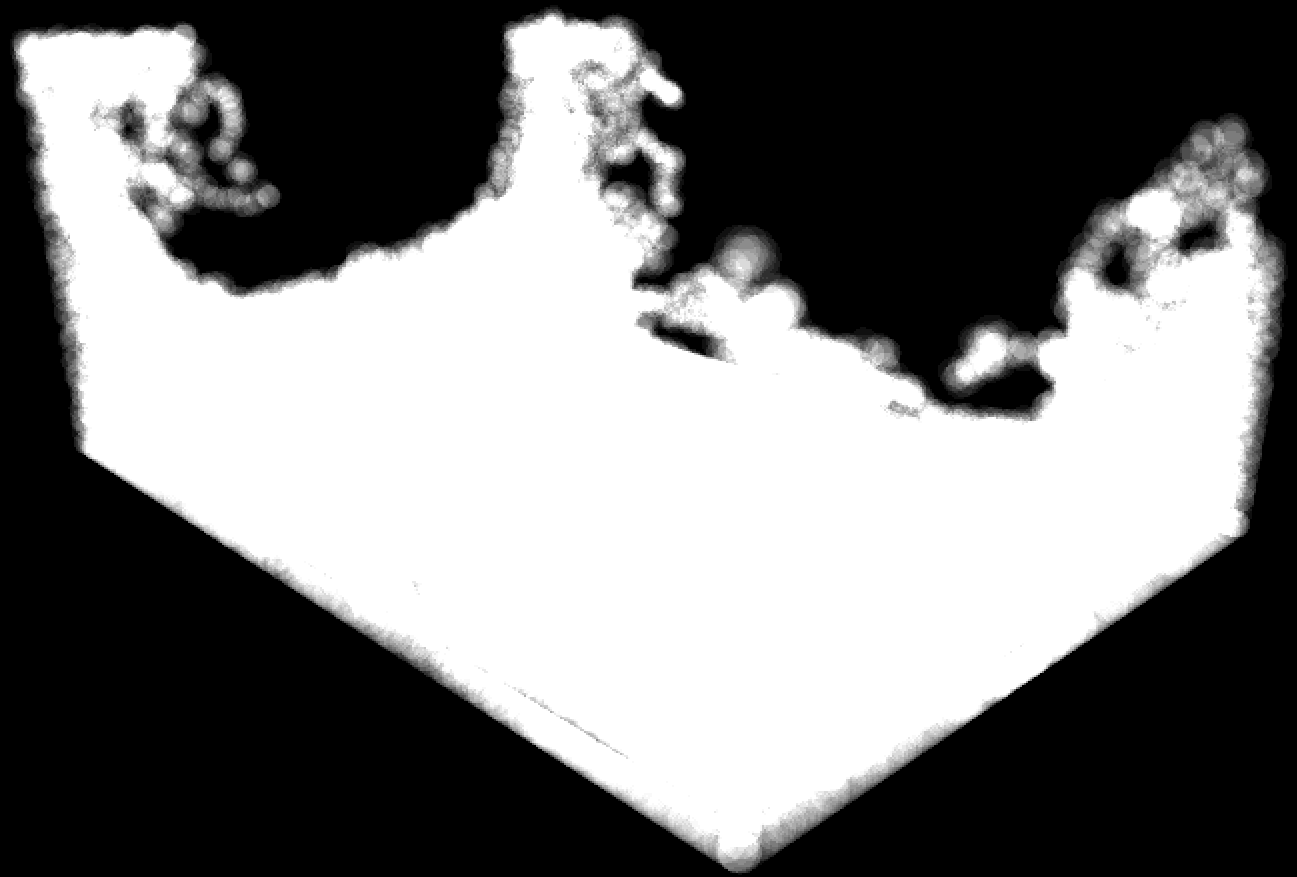
\includegraphics[width=.5\linewidth]{images/thicknessMap.png}}
    \caption{The particle thickness map.}\label{fig:thicknessmap}
\end{figure}
\noindent
Finally, to control the fluid's opacity and color, we compute its thickness and store the result in a texture. This is done by rendering all particles with OpenGL's additive blending enabled, so that the accumulated values in the texture represent fluid thickness, where 1 indicates maximum thickness and 0 indicates no fluid, as shown in Fig.\ref{fig:thicknessmap}. Depending on various factors, such as number of particles and screen resolution, this step can get very resource-intensive, therefore, in our implementation it is performed at half the resolution.

\subsection{Scene rendering and final composition}
\begin{figure}[ht!]
    \centering
        \subfloat[Refractions only]{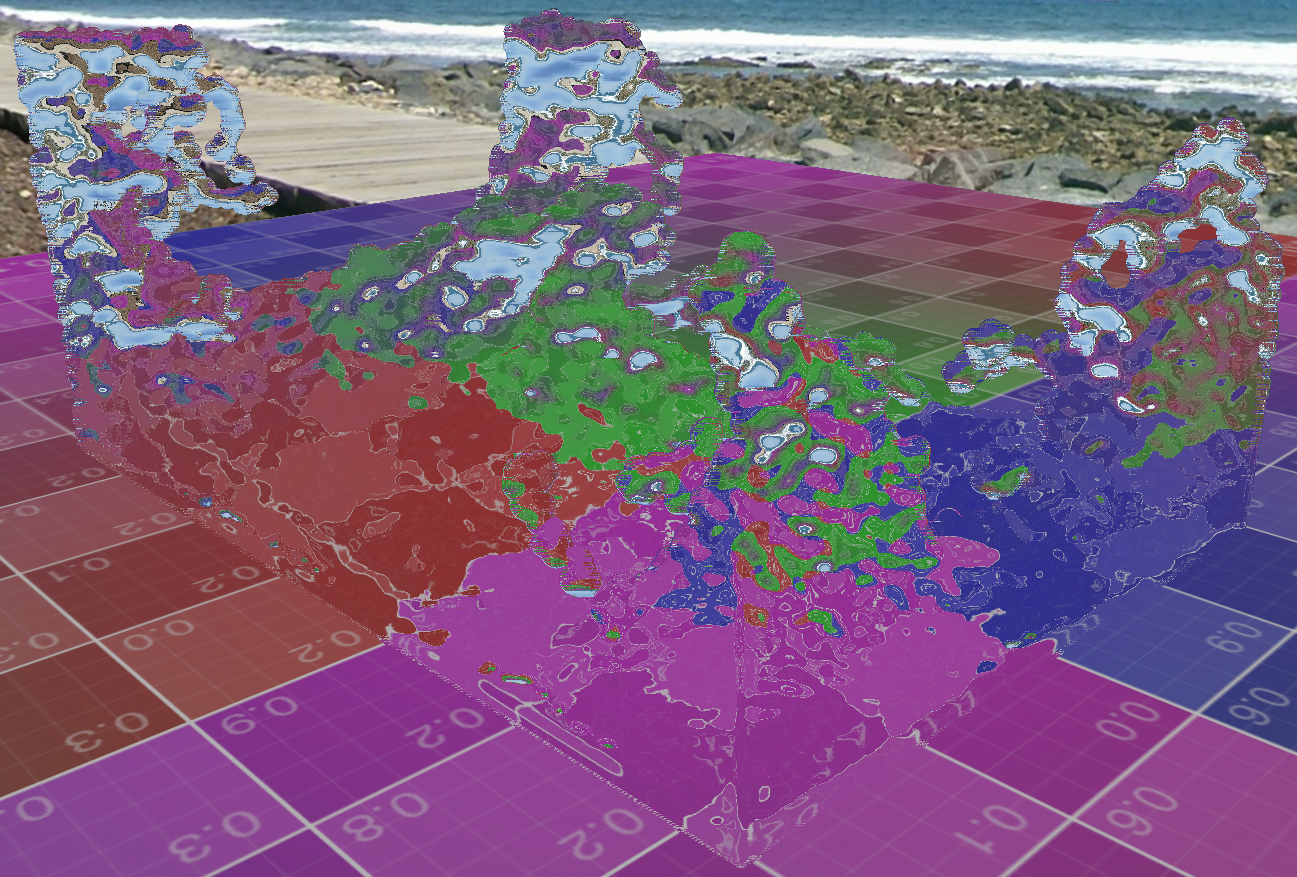
\includegraphics[width=.49\linewidth]{images/refractions.png}}\hfill
        \subfloat[Refractions + reflections + color]{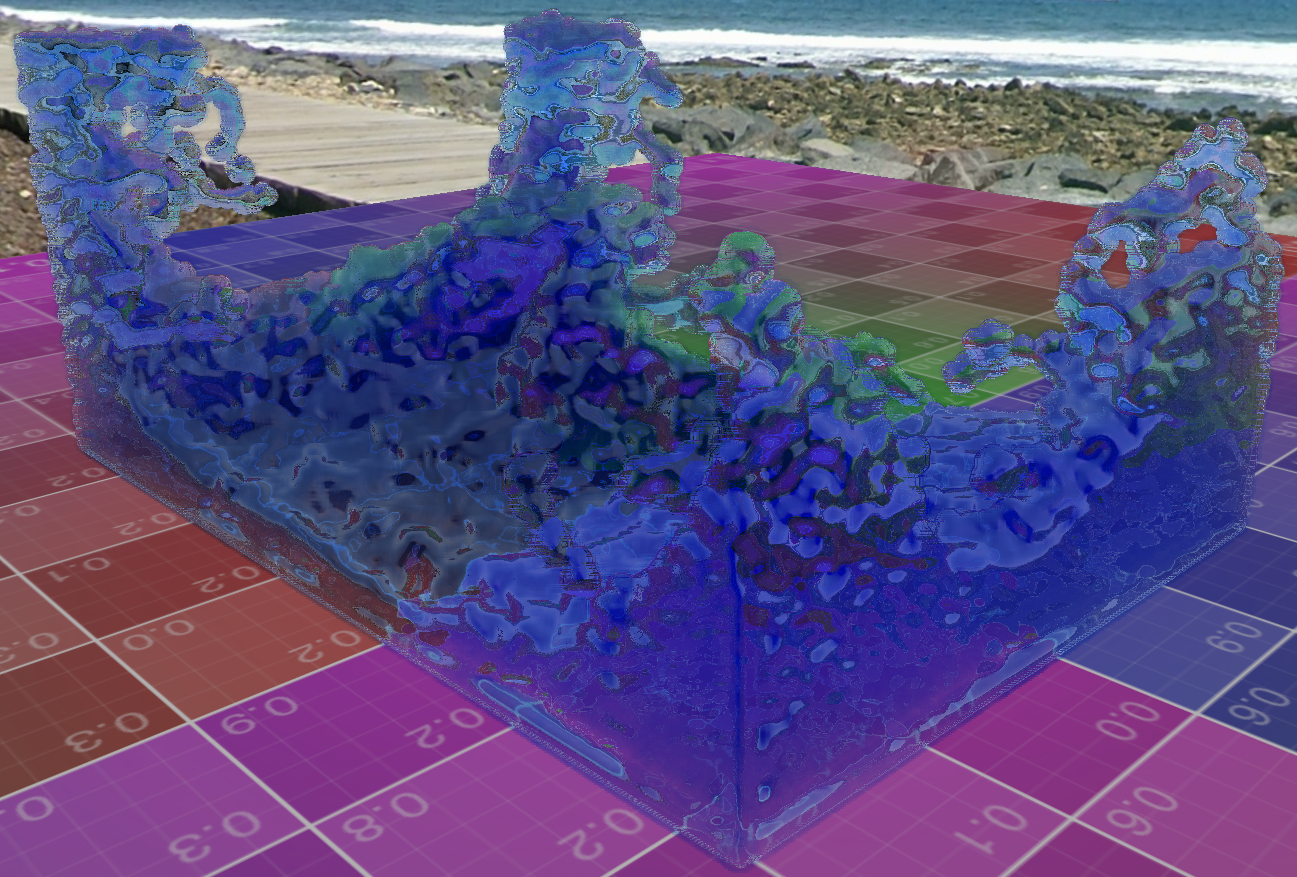
\includegraphics[width=.49\linewidth]{images/fluid_blue.png}}
    \caption{Final fluid rendering, with refractions only (a) and with reflections and light extinction coefficients set (b).}\label{fig:finalRenders}
\end{figure}

\noindent
The scene used in this project consists of a simple plane on which the fluid is located, and as a background, we used a generic cubemap\footnote{\url{https://www.humus.name/index.php?page=Cubemap&item=Tenerife2}}. The plane rendering is saved to a texture; this way when we compute refraction and reflection vectors we can easily check whether a ray-plane intersection occurs and sample either the plane texture or the cubemap accordingly. The main limitation of this approach is that, in case of more complex scenes, we need to update accordingly the ray-intersection tests, as well as the texture sampling logic.\\

\noindent
The final rendering steps can be summarized as follows:
\begin{itemize}
    \item \textbf{Refracted light}: after computing the refraction vector, sample the background texture (either the plane or the cubemap). Using the thickness texture and the color extinction coefficients of the fluid, we can compute its transmittance as follows:
    \begin{align}
        T &= \exp{(fluidColor \cdot thickness)}\\
        C &= C.rgb \odot T        
    \end{align}
    Here $T$ is the vector containing the transmittance coefficients for each color channel, and $C$ is the final color of the refraction ray.

    \item \textbf{Reflected light}: compute the reflection vector, sample the appropriate background texture.
    \item \textbf{Combine reflections and refractions}: we use the Schlick approximation \cite{schlick1994inexpensive} of the Fresnel reflectance equations to compute the reflection coefficient $\alpha$, and the resulting color is a linear interpolation of the reflected and refracted color: 
    \begin{align}
        F_0 &= \frac{(R_{air} - R_{water})^2}{(R_{air} + R_{water})^2} \\
        \alpha &= F_0 + (1-F_0)\cdot(1-\cos\theta)^5\\
        C &= \alpha\cdot C_{refraction} + (1-\alpha)\cdot C_{reflection}
    \end{align}
    Where $R_i$ is the Index of Refraction of a given material $i$, $\theta$ is the angle between the surface normal and the half vector, $C_{\{...\}}$ is the sampled background color, coming either from a reflection or a refraction. 
\end{itemize}

\noindent
By experimenting with the color extinction coefficients of the fluid, we can get the results shown in Fig.\ref{fig:finalRenders}b and Fig.\ref{fig:colors}.

\begin{figure}[ht!]
    \centering
        \subfloat{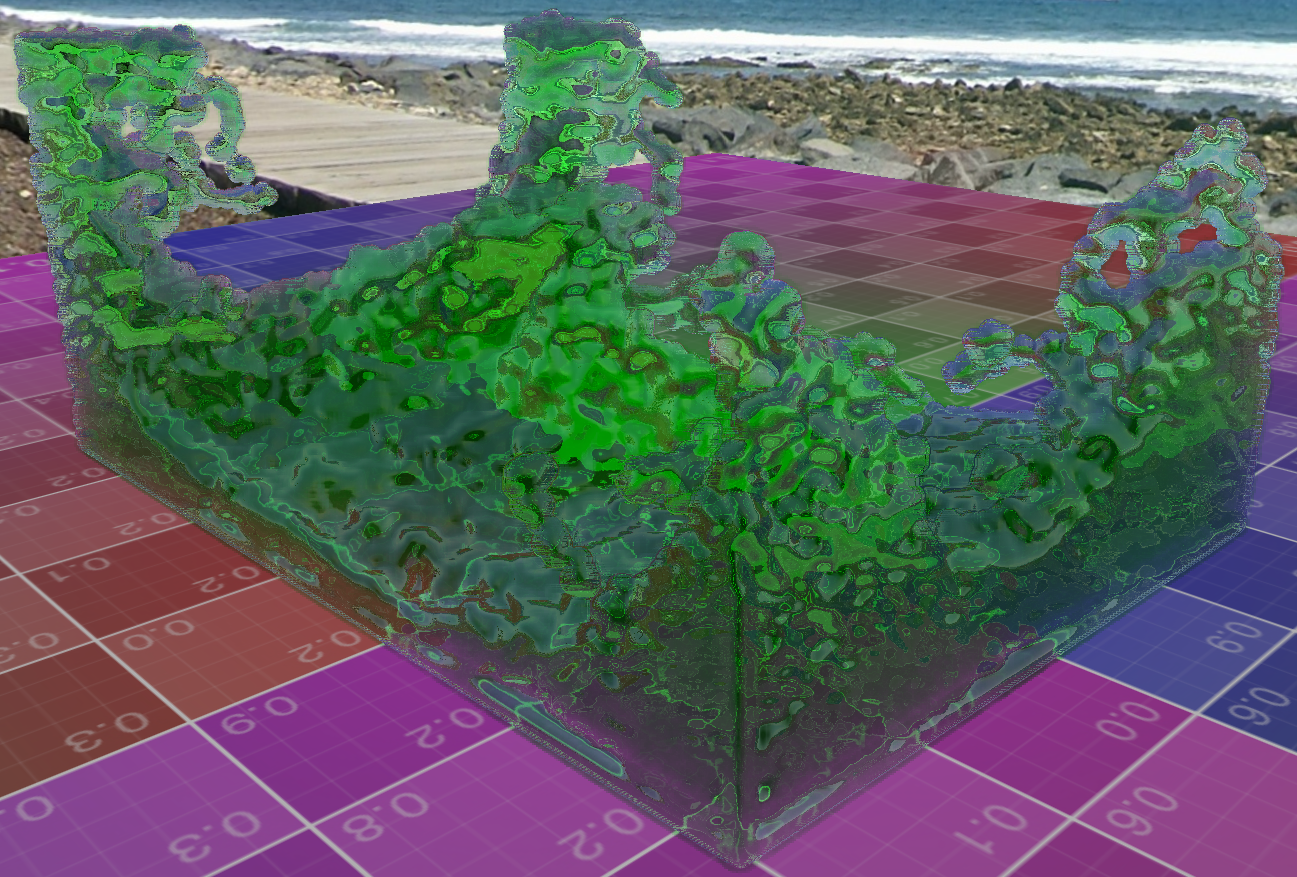
\includegraphics[width=.49\linewidth]{images/fluid_green.png}}\hfill
        \subfloat{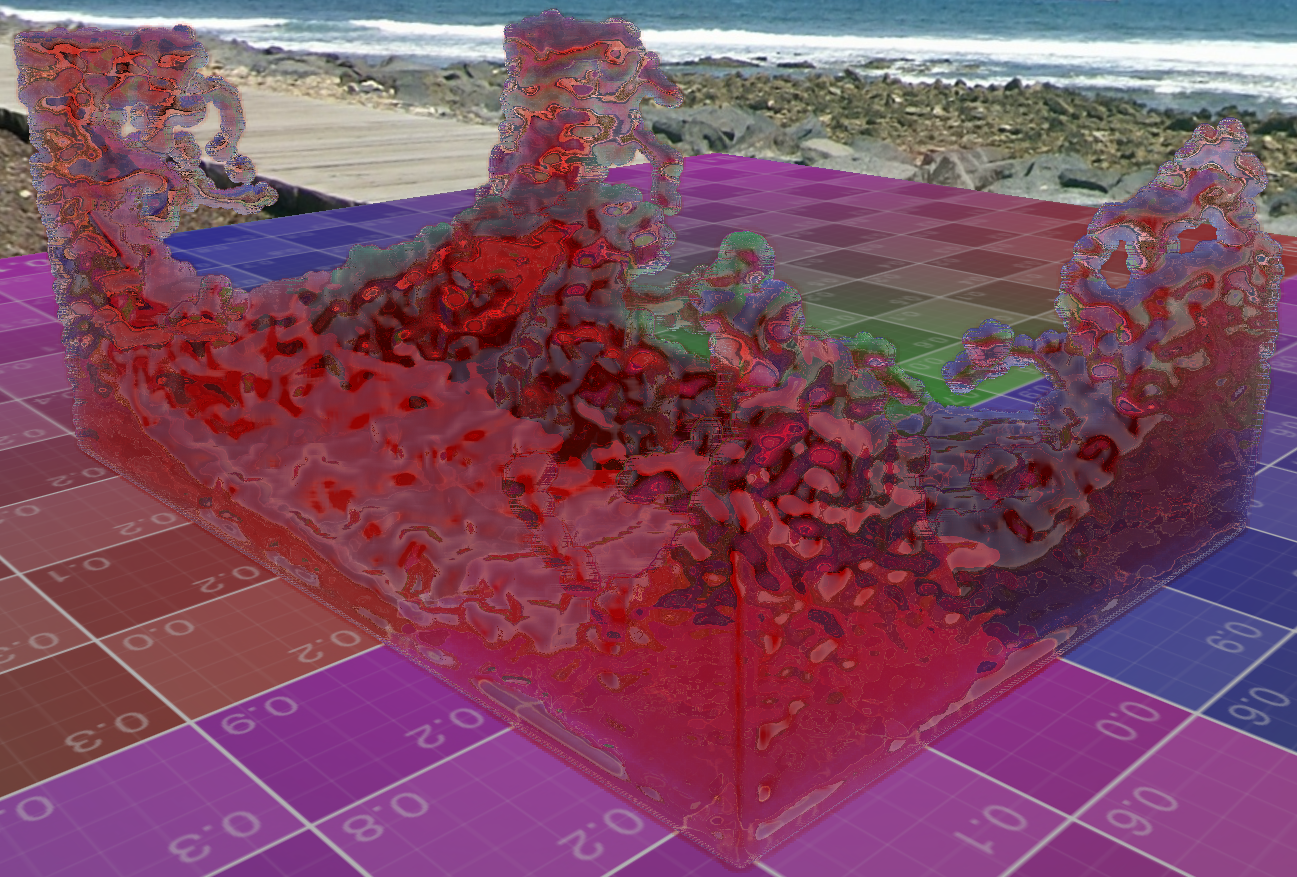
\includegraphics[width=.49\linewidth]{images/fluid_red.png}}
    \caption{Example of various fluid colors.}\label{fig:colors}
\end{figure}